\documentclass[11pt, a4paper]{article}
\usepackage{a4wide}
\usepackage{amsmath, amsfonts, dsfont, booktabs, graphicx, natbib, times, microtype, hyperref}
\newcommand{\E}{\ensuremath{{\mathbb E}}} % expected value
\def\func#1{\mathop{\rm #1}}
\begin{document}
\title{Solution to Exercise 4}
\author{Simon A.\ Broda}
\date{}
\maketitle

\begin{enumerate}
\item If we set $\alpha$ and $\beta_1$ to the same value, e.g., 1, then both series trend up by 1 each period. The correlograms look quite similar, but the time series plots don't really, even if we crank up the variance of the trend-stationary series. This is because the latter is stationary after de-trending (subtracting off $\beta_1\cdot t$, whereas the random walk with drift remains nonstationary if we subtract $\alpha\cdot t$ (it becomes a random walk without drift).
\item
\begin{enumerate}
\item The time series plot and the correlogram are shown below.
\begin{center}
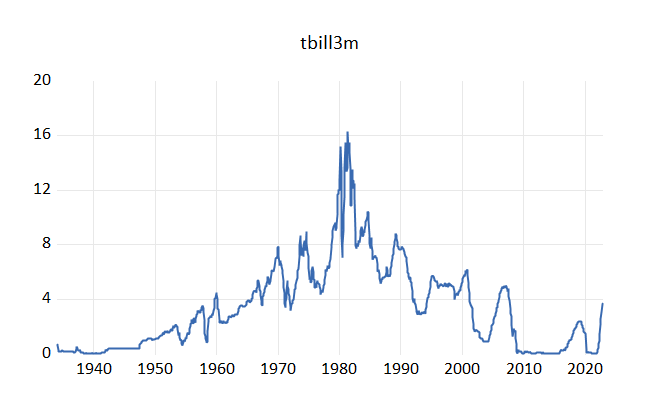
\includegraphics[width=.6\textwidth]{tbillplot}
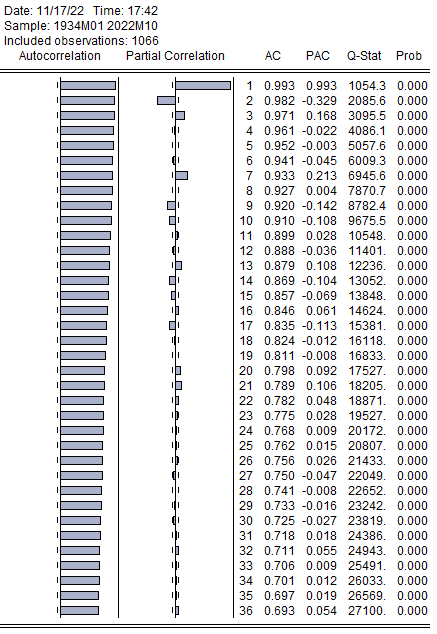
\includegraphics[width=.6\textwidth]{tbillcorr}
\end{center}
From the correlogram, it looks like the T-Bill rate is I(1): the autocorrelations are large and decay slowly and approximately linearly. We can confirm this with an ADF test: open the series and click on \texttt{View$\rightarrow$Unit Root Tests$\rightarrow$Standard Unit Root Test\ldots}. The data don't seem to have a trend\footnote{One could argue that there is a breaking trend, upwards \href{https://www.statista.com/statistics/1338105/volcker-shock-interest-rates-unemployment-inflation/}{until around 1982, downwards thereafter}, but this kind of test is not available in EViews.}, so we include just an intercept (because the mean is not zero). Choose automatic lag length selection, but switch to the AIC instead of the default BIC. This results in the following output.
\begin{center}
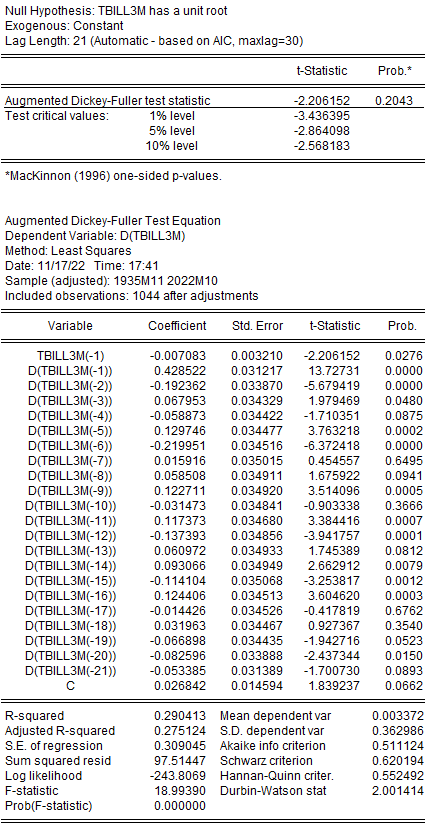
\includegraphics[width=0.6\textwidth]{tbilladf}
\end{center}
The observed test statistic is -2.206, larger than the critical value -2.86, so the test does not reject the null that the data are I(1), as expected. The same conclusion can be drawn from the $p$-value of 0.2043\footnote{Please be aware that in an exam, I might delete the top of the EViews output, and give you only the test regression at the bottom. Note that the $p$-value of the $t$-statistic there is wrong; it corresponds to the $p$-value from a standard regression with stationary variables, i.e., it's from a normal distribution instead of the Dickey-Fuller distribution. You can try this yourself by running the ADF regression manually, by entering \texttt{d(TBILL3M) c TBILL3M(-1) d(TBILL3M(-1)) \ldots TBILL3M(-21)} under \texttt{Quick$\rightarrow$Estimate Equation\ldots.}}.
\item We start by inspecting the correlogram of the first difference. This can either be done by creating a new series via \texttt{genr DTBILL3M = d(TBILL3M)} and inspecting its correlogram, or by opening \texttt{TBILL3M} (i.e., the series in levels), and then clicking \texttt{View$\rightarrow$\linebreak Correlogram...}, and specifying that you want the correlogram of the first difference.
\begin{center}
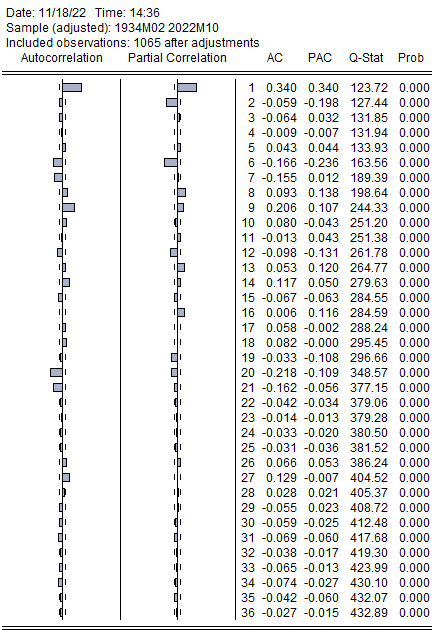
\includegraphics[width=.6\textwidth]{dtbillcorr}
\end{center}
The first difference looks stationary. After some specification search\footnote{\texttt{freeze(mode=overwrite, armatable) tbill3m.autoarma(tform=none, diff=1, select=sic, maxar=10, maxma=10, atable) forec c}}, we find that an ARMA(5, 5) model is the most adequate, even though it doesn't remove the autocorrelation completely. Estimating this model (either as \texttt{d(TBILL3M) c AR(1 to 5) MA(1 to 5)}, or if you created a new variable for the difference above, \texttt{DTBILL3M c AR(1 to 5) MA(1 to 5)}) yields the output and correlogram below.
\begin{center}
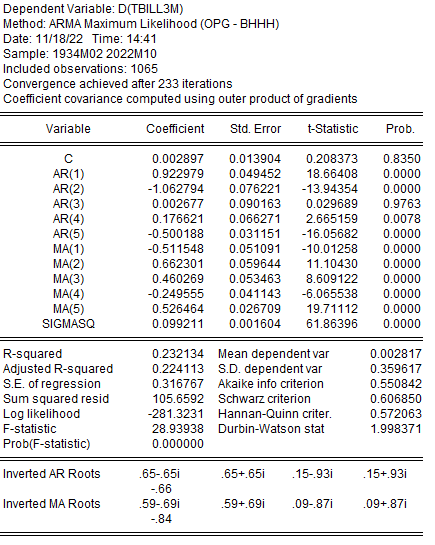
\includegraphics[width=0.6\textwidth]{arma55}
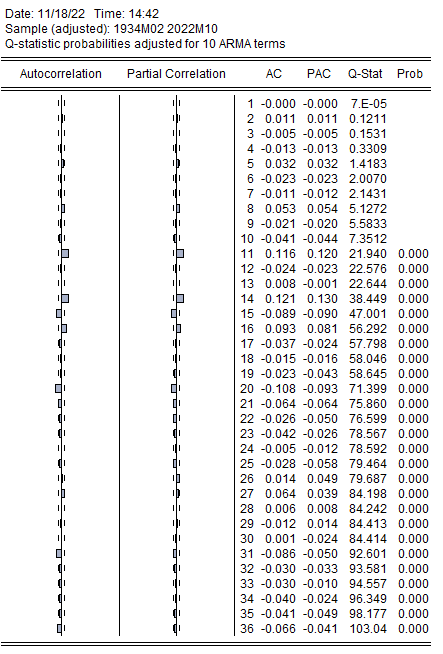
\includegraphics[width=0.6\textwidth]{arma55corr}
\end{center}
Some autocorrelation remains, but we won't bother to model it. So our final model for $\Delta$ TBILL3M is an ARMA(5, 5). This means that the levels TBILL3M follow an ARIMA(5, 1, 5) model.
\item To forecast an ARIMA model, we first forecast the ARMA model for the first difference. We'll spare us the hassle of doing a manual forecast for this complicated model, and just use EViews for it.  Extending the workfile to 2022M12 via \texttt{Proc$\rightarrow$Structure / Resize Current Page\ldots}, we can forecast by clicking \texttt{Forecast} on the estimated equation and setting the options as follows\footnote{Note that because I estimated my model using \texttt{d(TBILL3M) c AR(1 to 5) MA(1 to 5)}, EViews gives me the option to directly predict the levels, but we'll ignore this here.}:
\begin{center}
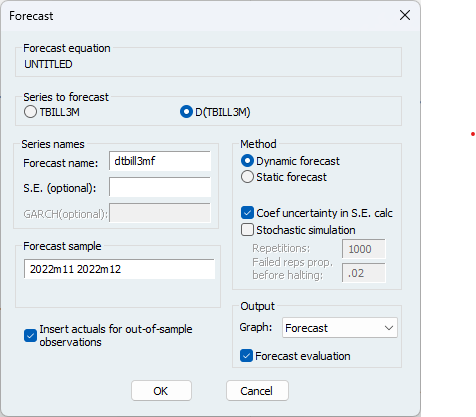
\includegraphics[width=0.6\textwidth]{forecast}
\end{center}
The forecasts are $\widehat{\Delta\mbox{TBILL}}_{2022M11}=0.1636$ and $\widehat{\Delta\mbox{TBILL}}_{2022M12}=-0.0328$. The T-Bill rate in 2022M10 was 3.72, so the corresponding forecasts for the levels are
\begin{align*}
\widehat{\mbox{TBILL}}_{2022M11}&=3.72+0.1636=3.8836\\
\intertext{and}
 \widehat{\mbox{TBILL}}_{2022M12}&=3.8836-0.0328=3.8508.
\end{align*}
\end{enumerate}
\item
\begin{enumerate}
\item We begin by creating the excess returns Note that the T-Bill rate is quoted in percent and in annualized terms, so we have to convert it to daily log returns first. The commands are
\begin{verbatim}
genr rf = log(1+dtb3/100)/365
genr r = dlog(ibm)-rf
genr rm = dlog(spx)-rf
\end{verbatim}
Running the CAPM regression of \texttt{r} on \texttt{rm} and an intercept results in the following output.
\begin{center}
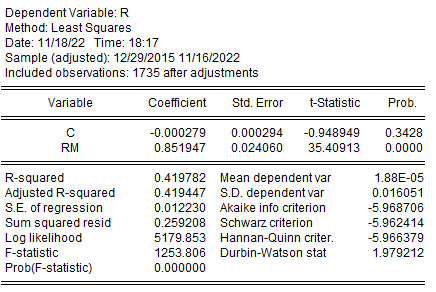
\includegraphics[width=0.6\textwidth]{capm}
\end{center}
The intercept (usually called $\alpha$) is insignificant as predicted by the theory, and the CAPM $\beta$ of IBM is $.852$.
\item The DW statistic is 1.9792. This value is between $d_u=1.78$ and 4, so we don't reject the null of no first order autocorrelation.
\item In the estimation output, go to \texttt{View$\rightarrow$Residual Diagnostics$\rightarrow$\linebreak Serial Correlation LM Test}, and include 5 lags. This results in the output below.
\begin{center}
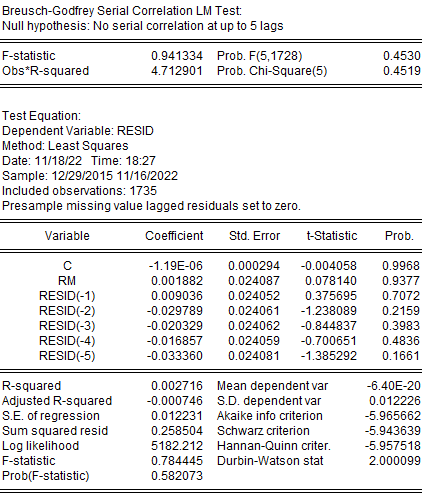
\includegraphics[width=0.6\textwidth]{breusch}
\end{center}
There are two versions of the test, the $F$-Test and the LM test. We'll focus on the LM test. The observed test statistic is $T\cdot R^2_{aux}=1735\cdot0.002716=4.71$, which doesn't exceed the critical value of 11.07 from the $\chi^2(5)$ distribution, so we don't reject the null of no serial correlation of order 5 or less. The same conclusion can be drawn from the top of the output, but that might get deleted in an exam.
\item Selecting HAC standard errors in the \texttt{Options} tab of the estimation window results in the following.
\begin{center}
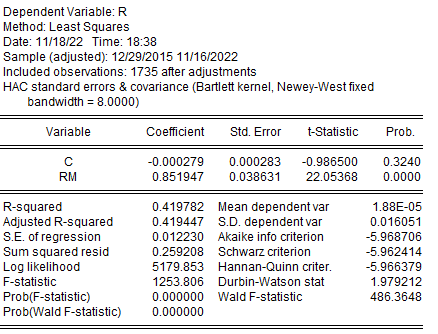
\includegraphics[width=0.6\textwidth]{hac}
\end{center}
As you can see, the difference isn't that big here, because there was little autocorrelation to begin with. Generally, if there is autocorrelation, then the HAC standard errors will be larger, i.e., the regular standard errors underestimate the variance of the estimates.
\end{enumerate}
\item
\begin{enumerate}

\item
For $Y_{1,t}$, we have
\begin{align*}
\E[\Delta Y_{1,t}]&=\E[Y_{1,t}-Y_{1,t-1}]\\
&=\E[\delta t+U_{1,t}-(\delta (t-1)+U_{1,t-1})]\\
&=\delta +\E[U_{1,t}-U_{1,t-1})]\\
&=\delta.
\end{align*}
For $Y_{2,t}$,
\begin{align*}
\E[\Delta Y_{2,t}]&=\E[Y_{2,t}-Y_{2,t-1}]\\
&=\E[\delta + Y_{2,t-1}+U_{2,t}-Y_{2,t-1}]\\
&=\E[\delta + U_{2,t}]\\
&=\delta.
\end{align*}
\item Consider the AR(2) process
\[
Y_t=\phi_1Y_{t-1}+\phi_2Y_{t-2}+U_t.
\]
We would like to test the null that $\phi_1+\phi_2=1$ (unit root) vs.\ $\phi_1+\phi_2<1$ (stationarity). This can be done by rearranging the equation as follows:
\begin{align*}
Y_t&=\phi_1Y_{t-1}+\phi_2Y_{t-2}+U_t&\mid&-Y_{t-1}\\
Y_t-Y_{t-1}&=(\phi_1-1)Y_{t-1}+\phi_2Y_{t-2}+U_t&\mid&\pm \phi_2Y_{t-1}\\
Y_t-Y_{t-1}&=(\phi_1-1)Y_{t-1}+\phi_2Y_{t-1}-\phi_2Y_{t-1}+\phi_2Y_{t-2}+U_t\qquad&\\
Y_t-Y_{t-1}&=(\phi_1+\phi_2-1)Y_{t-1}-\phi_2\Delta Y_{t-1}+U_t&\\
\Delta Y_t&=\psi Y_{t-1}+\alpha_1\Delta Y_{t-1}+U_t,&
\end{align*}
where $\psi:=(\phi_1+\phi_2-1)$ and $\alpha_1:=-\phi_2$. Thus testing $\phi_1+\phi_2=1$ vs.\ $\phi_1+\phi_2=<1$ is equivalent to testing $\psi=0$ vs.\ $\psi<0$ in a regression of
$\Delta Y_t$ onto $Y_{t-1}$, augmented by one lag of $\Delta Y_{t-1}$.

\end{enumerate}


\end{enumerate}
\end{document} 